% Origen: Secciones/PI - Resultados de Merito.md (antes "... Merito MCA")
% (antes "PI - Resultados de Monte-Carlo, Validacion y Mediciones"). La parte de
% Monte-Carlo quedó en otra nota, "PI - Resultados Monte - Carlo.md", todavía
% sin convertir: por eso S:res-montecarlo sigue pendiente en cap4.
\chapter{Resultados de mérito}
\label{C:resultados}

% Figuras de ESTE capítulo + las compartidas. Siempre al principio del archivo.
\graphicspath{{figs/cap9/}{figs/comunes/}}

\begin{destacado}
En este capítulo se presentan resultados de mediciones mediante la generación
interna y posterior canalización a un lazo analógico del módulo MCA.
\end{destacado}

%==============================================================================
\section{Etapas de experimentos y validación}
\label{S:res-etapas-validacion}

Esto es aislar las dependencias en la cadena de adquisición; en particular
identificamos las siguientes:
\begin{itemize}
  \item \textbf{Simulación} (Monte-Carlo):
  \begin{itemize}
    \item Completamente computacional.
    \item No necesariamente contiene detalles de la implementación del HW.
  \end{itemize}
  \item \textbf{Verificación}: simulaciones de comprobación de la respuesta del
    HW.
  \begin{itemize}
    \item Nuestros estímulos se realizan mediante asignaciones directas a las
      señales de entrada de un módulo; estas operaciones no son sintetizables.
    \item Estos resultados se presentan en las secciones de verificación de los
      módulos individuales, por ejemplo la Sec.~\ref{S:ap-mt-verificacion}.
  \end{itemize}
  \item \textbf{Generación interna}:
  \begin{itemize}
    \item Ya estamos de forma completa en HW.
    \item Medimos en HW una salida generada por el mismo HW. Un ejemplo de la
      misma se encuentra en la
      Fig.~\ref{f:top-datapath}.
    \item La señal generada tendrá las propiedades que nosotros deseamos: vamos
      a tener una emisión de un comando de generación y vamos a ver la salida de
      nuestros módulos a la misma.
  \end{itemize}
  \item \textbf{Generación externa controlada}:
  \begin{itemize}
    \item Los comandos de generación se transmiten a un elemento externo, como
      un generador de pulsos, y la salida de este se conecta a nuestro HW por
      una interfaz rápida. Esto se presenta en la
      Fig.~\ref{f:res-setup-externo}.
  \end{itemize}
  \item \textbf{Medición con \emph{setup} experimental}: utilizamos un medidor con
    física real.
\end{itemize}

%==============================================================================
\section{Resultados de generación externa controlada}
\label{S:res-gen-externa}

Este fue el primer sistema de medición real que implementamos. Conectamos las
dos entradas analógicas de alta velocidad a los dos canales de salida del
generador de ondas Rigol DG-4162. Ambas conexiones utilizaban un coaxial
KingSignal RG-58 con conectores macho SMA en las terminales de la Pitaya y
conector BNC en la terminal del Rigol. El Rigol se controló por su puerto
trasero del tipo USB-Host, manejado por la Pitaya; la comunicación se realizó
mediante el protocolo especializado Rigol USB TMC \emph{Driver}. En la
Fig.~\ref{f:res-setup-externo} se presenta de forma esquemática el \emph{setup};
mediante \codigo{ssh} teníamos control de los \emph{scripts} de testeo.

\begin{figure}[H]
\centering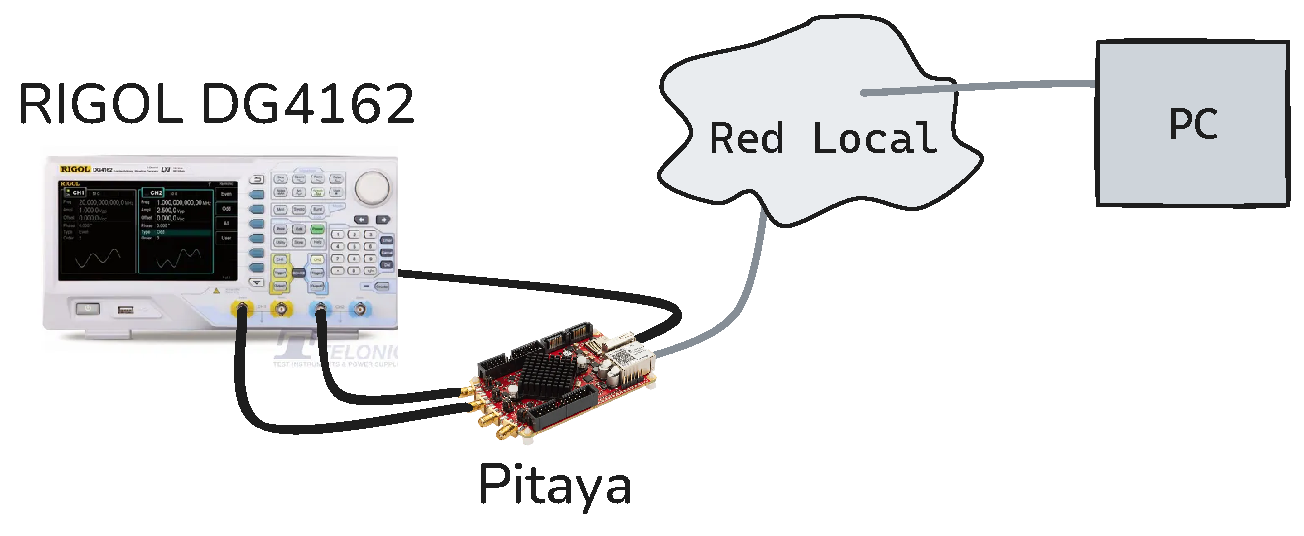
\includegraphics{cap9_setup_externo}
\caption[Esquema de verificación inicial]{%
Esquema de verificación inicial.\label{f:res-setup-externo}}
\end{figure}

Aún así, este sistema cuenta con las siguientes limitaciones:
\begin{itemize}
  \item Techo de \emph{throughput}: la generación de pulsos con este sistema
    tiene como límite 794~kEv/s.
  \item No separa la INL del generador de la del ADC: la entrada es la cascada
    de los dos sistemas.
\end{itemize}
Para superar estas limitaciones pasamos a la configuración de generación
interna.

\subsection{\emph{Setup} de generación interna}
\label{S:res-setup-interna}

La versión más simple de realizarla es mediante el lazo interno a la PL:
ponemos en la entrada de nuestros medidores la salida de un módulo que genera
estímulos controlados (\codigo{gen\_pulsos}), y a esto lo llamamos \textbf{lazo
digital}. El \textbf{lazo analógico}, en cambio, canaliza la salida del ASG al
OUT1 de la Pitaya, que se conecta a IN1. En este caso testearíamos el sistema
anterior más los efectos producidos por los front-end analógicos, el ADC, el
DAC, las terminaciones SMA y el cable coaxial. Este \emph{setup} se puede observar en
la Fig.~\ref{f:res-conexion-in-out}.

\begin{figure}[H]
\centering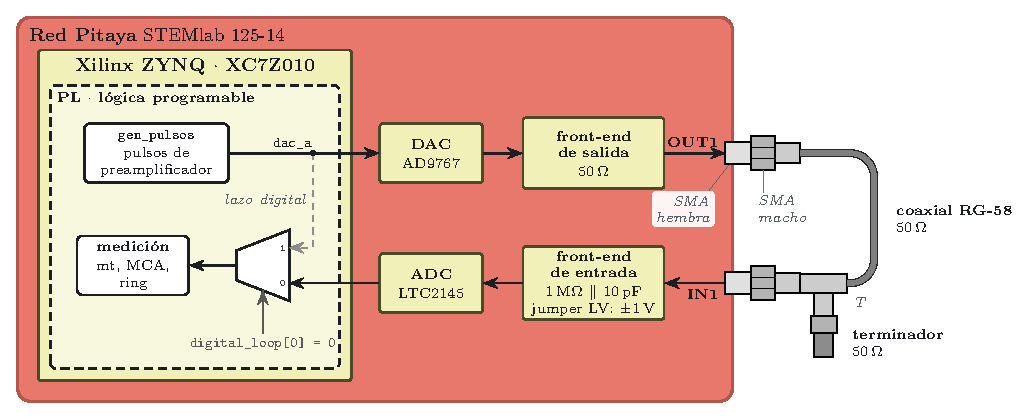
\includegraphics{cap9_conexion_in_out}
\caption[\emph{Setup} de generación interna]{%
\emph{Setup} de generación interna. Se puede emplear \codigo{digital\_loop=1} para que
la señal se genere y se consuma dentro del \emph{fabric} de la PL, o se puede utilizar
\codigo{digital\_loop=0} para hacer uso de la entrada analógica \codigo{IN1}, en
este caso conectada directamente desde OUT1 con un conector T y una carga de
\qty{50}{\ohm}.\label{f:res-conexion-in-out}}
\end{figure}

Conectamos OUT1 a IN1 con una T y una carga de \qty{50}{\ohm} porque, si no, se
presentaban los armónicos lentos en \qty{12.3}{\mega\hertz},
\qty{34.7}{\mega\hertz} y \qty{53.2}{\mega\hertz} mostrados en la
Fig.~\ref{f:res-canal}(b), que es la transferencia para OUT2 $\rightarrow$ IN2
sin compensación. Para el resto de las pruebas se utilizó el canal
OUT1 $\rightarrow$ IN1 adaptado.

\begin{figure}[H]
\centering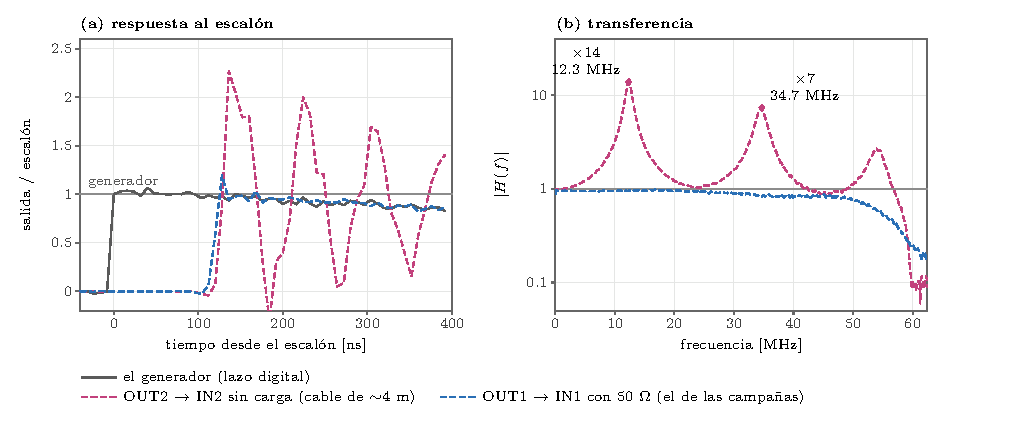
\includegraphics{cap9_canal_analogico}
\caption[El canal analógico medido con la BRAM]{%
El canal analógico medido con la BRAM: el mismo estímulo capturado con el lazo
digital (el generador) y sin él. (a) Respuesta a un escalón de 1727~ADU,
normalizada; (b) transferencia $|H(f)|$ por espectros cruzados
(Welch).\label{f:res-canal}}
\end{figure}

\begin{destacado}
Las amplitudes no las expresamos en tensión sino en \textbf{ADU}
(\emph{analog-to-digital units}), el escalón del código de 14 bits. Las
posiciones en el histograma (centroides y corrimientos) van en
\textbf{canales}.
\end{destacado}

%==============================================================================
\section{Resultados de generación interna}
\label{S:res-gen-interna}

Una vez comprobado el funcionamiento correcto de la fuente de pulsos comenzamos
a realizar diversas pruebas; en la Tabla~\ref{t:res-setup} se presenta la
configuración del MCA en las mediciones. Se denominan \textbf{pulsos buenos} los
estimados dentro de un rango de \qty{2}{\percent} de error.

% La tabla no tiene epígrafe en la nota y la frase que la presenta quedó
% cortada ("en la Tabla{prueba_setup_original} las mediciones ."): el epígrafe
% y el "se presenta la configuración del MCA" son provisorios.
\begin{table}[H]
\centering
\caption[Configuración del MCA en las mediciones]{%
Configuración del MCA en las mediciones de generación
interna.\label{t:res-setup}}
\begin{tabularx}{\textwidth}{|l|>{\raggedright\arraybackslash}X|}
\hline \encabezado \textbf{Parámetro} & \textbf{Valor} \\ \hline
Espectro 1D & 8192 canales (\codigo{H\_AW} = 13), contadores de 32 bits que
  saturan \\ \hline
Mapa 2D & $128 \times 64$ canales (amplitud $\times$ forma) \\ \hline
Ranuras de medición & 3 (\codigo{N\_ACC}) \\ \hline
Formas del banco de trapecios & 3 (\codigo{N\_FORMAS}) \\ \hline
\end{tabularx}
\end{table}

\subsection{Comparación de la tasa de medición obtenida vs.\ la excitada}
\label{S:res-tasa}

Para medir la tasa de eventos, hicimos un barrido de la tasa de entrada de
10~k/s a 3~M/s. Los arribos son de Poisson, con dos líneas de 500 y 1300
cuentas (60/40) y $\tau = \qty{2}{\micro\second}$. Los resultados con el ASG y
de 1 a 3 ranuras se presentan en la Fig.~\ref{f:res-tasa}. Con 3 ranuras y
3~M/s de entrada, el MCA acepta 1.9~M/s y entrega 1.2~M/s buenos.

\begin{figure}[H]
\centering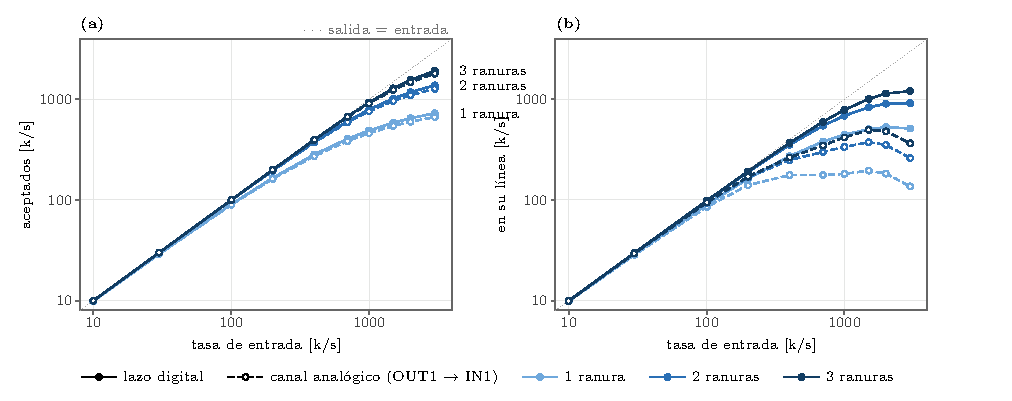
\includegraphics{cap9_meritos_tasa}
\caption[Tasa de eventos del MCA contra la cantidad de ranuras]{%
Tasa de eventos del MCA con \codigo{gen\_pulsos} (Poisson, líneas de 500 y
1300~ADU, disparo por el ASG, trapecio). (a) Eventos aceptados por segundo y
(b) eventos en su línea (a $\pm\qty{2}{\percent}$ del centroide de su línea de
referencia) por segundo, contra la tasa de entrada, con 1, 2 y 3 ranuras. Línea
llena: lazo digital; a trazos: canal analógico OUT1 $\rightarrow$ IN1 con
\qty{50}{\ohm}.\label{f:res-tasa}}
\end{figure}

\textbf{En el canal analógico los aceptados casi no cambian, pero la tasa en la
línea cae.}

Si realizamos la misma medición pero cambiando las fuentes de disparo obtenemos
la Fig.~\ref{f:res-tasa-fuentes}.

\begin{figure}[H]
\centering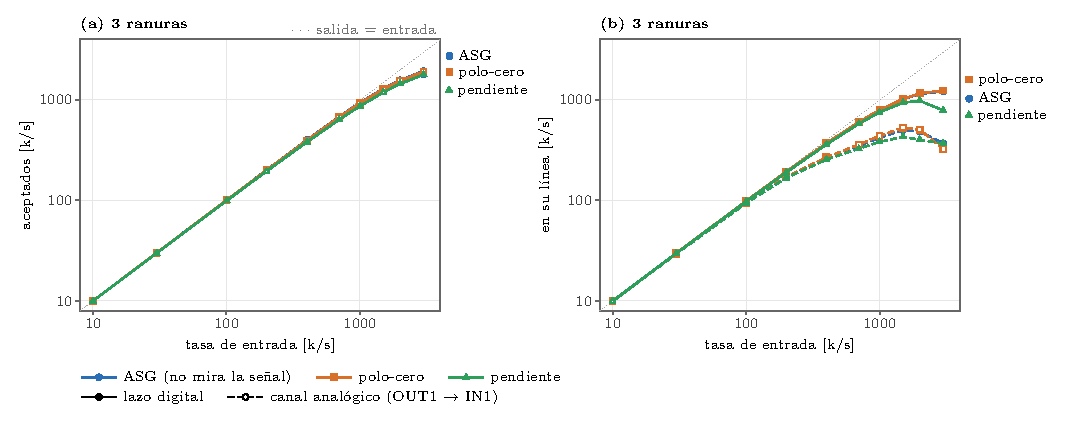
\includegraphics{cap9_meritos_tasa_fuentes}
\caption[Tasa de eventos con cada fuente de disparo]{%
Tasa de eventos con cada fuente de disparo (Poisson, líneas de 500 y 1300~ADU,
disparo por el ASG, trapecio). (a) Eventos aceptados y (b) eventos en su línea
(a $\pm\qty{2}{\percent}$ del centroide de su línea de referencia) por segundo,
contra la tasa de entrada. Línea llena: lazo digital; a trazos: canal analógico
OUT1 $\rightarrow$ IN1 con \qty{50}{\ohm}.\label{f:res-tasa-fuentes}}
\end{figure}

El ASG refiere a la salida del generador de pulsos que indica cuándo un pulso
sale del sistema; un \emph{trigger} ideal debería ser igual a esta ciclo a ciclo (a
menos de un retardo fijo).

\subsection{Error de tasa estimada}
\label{S:res-error-tasa}

En la Sec.~\ref{S:res-tasa} vimos la \textbf{tasa medida}; ahora podemos aplicar
sobre esta una compensación para obtener un \textbf{estimador de la tasa real}
$\hat\lambda$. Este mecanismo se presenta en el Cap.~\ref{C:implmca}.
A esta la comparamos con la tasa exacta del generador. Los resultados se
presentan en la Fig.~\ref{f:res-lambda}, como error relativo en \%, con 1
ranura en (a) y 3 ranuras en (b).

\begin{figure}[H]
\centering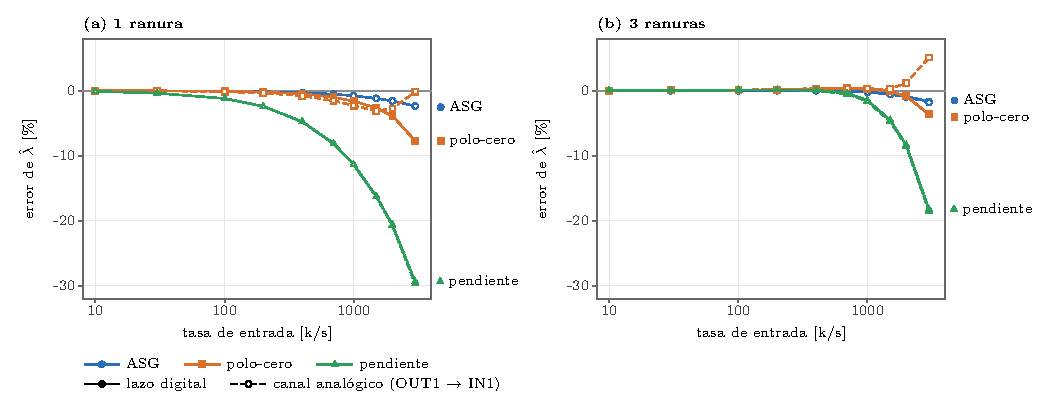
\includegraphics{cap9_meritos_lambda}
\caption[Error de la tasa estimada por el MCA]{%
Error de la tasa estimada por el SW del MCA medida contra la tasa del
generador.\label{f:res-lambda}}
\end{figure}

\subsection{Medición de la resolución de pico en función del ruido}
\label{S:res-ruido}

Para medir la resolución de cada estimador, hicimos un barrido de la varianza
del ruido blanco que suma \codigo{gen\_pulsos}, de 0 a 148~ADU de $\sigma$
(\codigo{ruido\_sh} de 8 a 0). La línea es de 1500~ADU, con 4000 pulsos por
punto. Usamos el disparo del ASG, que no depende del ruido. Ajustamos la curva
\begin{equation}
  \sigma^2 = (g\,\sigma_\text{ruido})^2 + \sigma_0^2 ,
  \label{e:res-ruido}
\end{equation}
donde definimos $g$ como la ganancia de ruido del estimador y $\sigma_0$ como el
ruido de fondo. Los resultados se presentan en la Fig.~\ref{f:res-ruido}, con
los dos ejes logarítmicos.

\begin{figure}[H]
\centering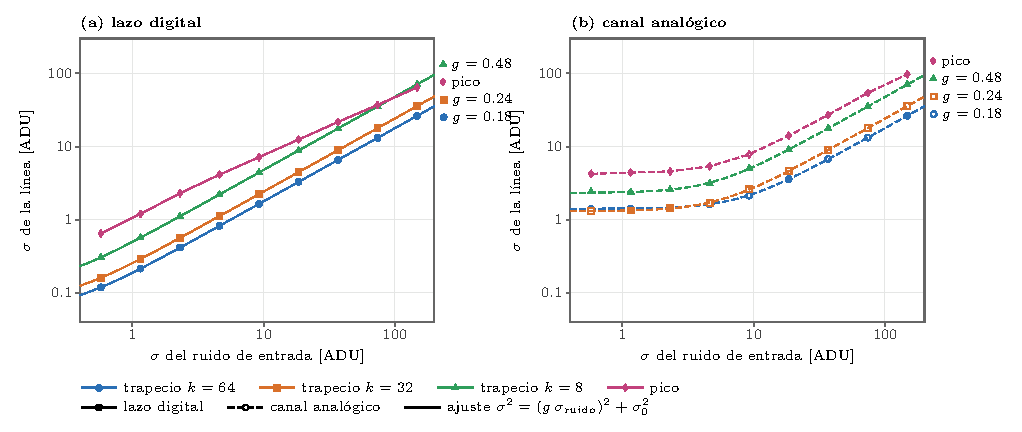
\includegraphics{cap9_meritos_ruido}
\caption[Resolución de cada estimador contra el ruido blanco]{%
Resolución de cada estimador contra el ruido blanco que suma
\codigo{gen\_pulsos} (línea de 1500~ADU, disparo por el ASG, 4000 pulsos por
punto): $\sigma$ de la línea, en ADU, contra el $\sigma$ del ruido de entrada.
Las curvas son el ajuste
$\sigma^2 = (g\,\sigma_\text{ruido})^2 + \sigma_0^2$.\label{f:res-ruido}}
\end{figure}

La ganancia de ruido $g$ baja con la subida $k$ del trapecio como $1/\sqrt{k}$
(0.48, 0.24 y 0.18 para $k = 8$, 32 y 64) y es la misma en los dos modos; el
canal analógico agrega el piso $\sigma_0$ del ADC.

% Desde acá las figuras van con [H]: el texto es corto y como floats se
% acumulaban al final del capítulo, solas en sus páginas.
\subsection{Medición de la resolución de par de pulsos y sobreestimación de
  pulsos}
\label{S:res-par}

Para medir la resolución de pulsos dobles, generamos pares de 4000 y 2400
cuentas y barrimos la separación $\Delta t$ entre ellos de 2 a 512 ciclos de
\qty{8}{\nano\second}, con 2000 pares por punto. Con 1 ranura, los dos pulsos
salen bien recién desde $\Delta t = 192$. La resolución fija la ranura: el
segundo pulso tiene que esperar a que se libere. En el canal analógico, la
pendiente se comporta igual. El polo-cero, en cambio, vuelve a disparar sobre el
sobrepico del \qty{24}{\percent}, con hasta 3.8 disparos por par, y casi nunca
deja los dos pulsos buenos (Fig.~\ref{f:res-par}).

\begin{figure}[H]
\centering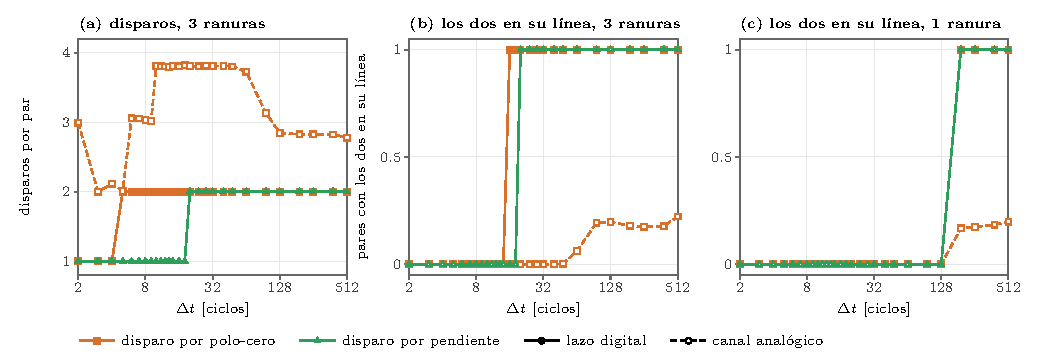
\includegraphics{cap9_meritos_par}
\caption[Resolución de pulsos dobles]{%
Resolución de pulsos dobles: pares de 4000 y 2400~ADU separados $\Delta t$
ciclos de \qty{8}{\nano\second}, 2000 pares por punto. (a) Disparos por par;
(b) fracción de pares en que el trapecio mide los dos pulsos en su línea
($\pm\qty{2}{\percent}$) con 3 ranuras y (c) con 1 ranura.\label{f:res-par}}
\end{figure}

\subsection{Medición del corrimiento del centroide}
\label{S:res-corrimiento}

Para el mismo barrido de tasa comparamos la posición del centroide emitido con
el medido, en búsqueda de \textbf{desviaciones sistemáticas}. Los resultados se
presentan en la Fig.~\ref{f:res-corrimiento}, con una curva por línea.

\begin{figure}[H]
\centering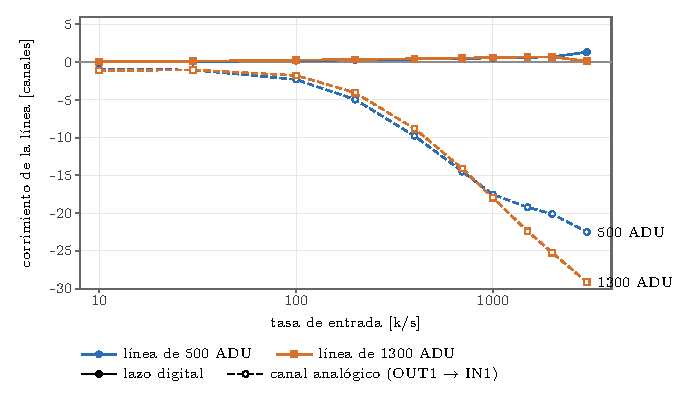
\includegraphics{cap9_meritos_corrimiento}
\caption[Corrimiento del centroide contra la tasa de entrada]{%
Corrimiento del centroide de cada línea contra la tasa de entrada (trapecio,
ASG, 3 ranuras, base fija). En el lazo digital no tenemos corrimiento
apreciable hasta 1~MEv/s, donde se vuelve menor de 2
canales.\label{f:res-corrimiento}}
\end{figure}

En el lazo digital las líneas no se mueven más de 2 canales; el canal analógico,
por otro lado, tiene un error que sigue la misma ecuación que vimos antes
\incompleto{} (falta la ecuación del error). Aún así, este elemento no es
corregible porque no es interno a nuestro módulo. Nos habla de la transferencia
analógica del canal. Por esta razón se recomienda
realizar esta medición previa para obtener la curva de respuesta del
corrimiento y poder compensar de forma automática según los valores obtenidos.
Es importante, igualmente, utilizar el mismo conexionado del \emph{setup} con el que
estemos trabajando, pero en vez de utilizar como salida el sensor, conectar a
OUT1.

\begin{destacado}
Estas \textbf{desviaciones se explican por el apilamiento} sobre las colas
negativas que deja la caída lenta del canal: la base baja con la tasa, y el
trapecio con polo-cero pasa ese error a la amplitud en $(k + m)/\tau$, igual
para todas las alturas hasta $\sim$1~M/s, donde el banco pasa a las formas
cortas.
\end{destacado}

\subsection{Medición de la no linealidad integral (INL) del conformado
  trapezoidal}
\label{S:res-inl-trapecio}

Con los mismos pulsos aislados medimos la línea del trapecio en cada amplitud.
Ajustamos una recta entre 200 y 3200~ADU, donde nada satura, y calculamos el
residuo en \% del fondo de escala (8191~ADU). Los resultados se presentan en la
Fig.~\ref{f:res-inl}. En el lazo digital, el residuo es menor que
\qty{0.002}{\percent}~FS (0.16~ADU) en todo el rango.

\begin{figure}[H]
\centering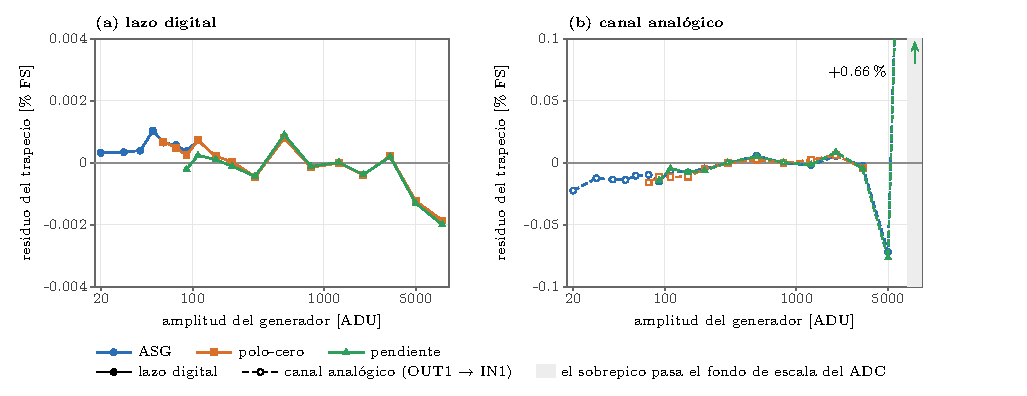
\includegraphics{cap9_meritos_inl}
\caption[No linealidad integral del trapecio]{%
No linealidad integral del trapecio, con cada fuente de disparo: el residuo de
la línea de pulsos aislados (400 por amplitud) contra una recta ajustada entre
200 y 3200~ADU, en \% del fondo de escala (8191~ADU). (a) Lazo digital, (b)
canal analógico.\label{f:res-inl}}
\end{figure}

El polo-cero no tiene línea desde 5000~ADU, porque vuelve a disparar sobre el
sobrepico; este efecto de disparo se presenta en la Sec.~\ref{S:res-walk}.

\subsection{Medición del \emph{walk} de disparo}
\label{S:res-walk}

Para medir el umbral y el \emph{walk} de cada fuente de disparo, barrimos la amplitud
de pulsos aislados de 20 a 8000~ADU, con 400 pulsos por punto y un ruido de
2.3~ADU. Los resultados se presentan en la Fig.~\ref{f:res-walk}. En cada punto
medimos tres cosas. La curva del panel (a) da la fracción de pulsos que disparan
y nos dice el umbral efectivo a utilizar. El polo-cero dispara la mitad de los
pulsos en 48~ADU y la pendiente en 81. En el canal analógico, 51 y 82: el canal
casi no mueve el umbral. El panel (b) es el \emph{walk}, el retardo del disparo, a
partir de \codigo{t\_subida}. El polo-cero se atrasa 1 ciclo
(\qty{8}{\nano\second}) con los pulsos chicos y la pendiente 6 ciclos
(\qty{48}{\nano\second}). En el canal analógico, 2 y 6.9 ciclos. En el panel
(c) están los disparos por pulso: el ASG dispara una vez siempre, porque no mira
la señal. En el canal analógico, el polo-cero vuelve a disparar \textbf{sobre el
sobrepico desde unas 3200~ADU}.

\begin{figure}[H]
\centering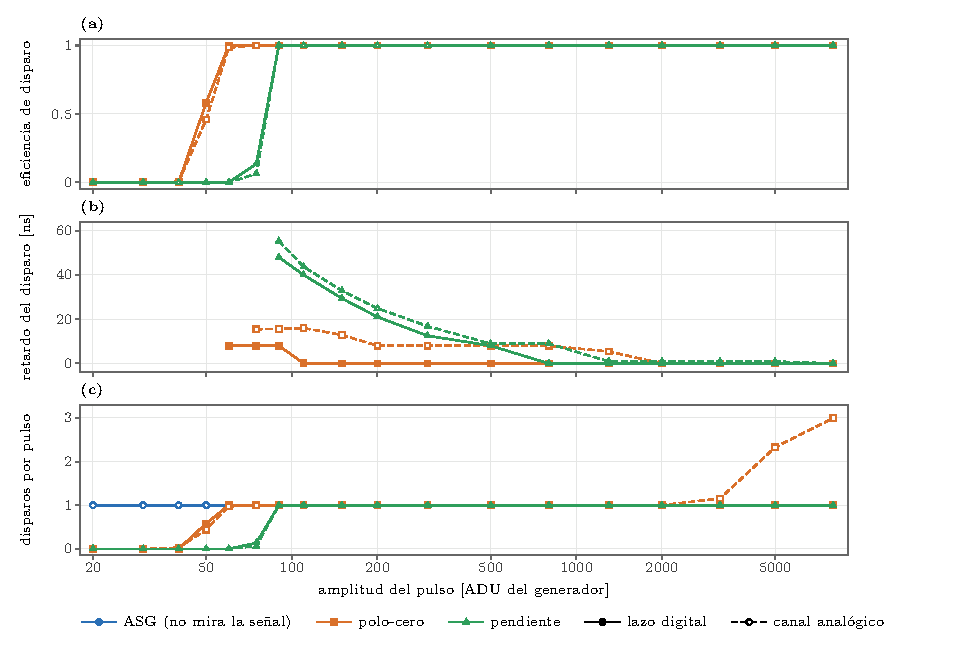
\includegraphics{cap9_meritos_walk}
\caption[El disparo contra la amplitud de un pulso aislado]{%
El disparo contra la amplitud de un pulso aislado (400 pulsos por punto, ruido
de 2.3~ADU). (a) Fracción de pulsos que disparan, (b) retardo del disparo, en
ciclos de \qty{8}{\nano\second}, (c) disparos por pulso.\label{f:res-walk}}
\end{figure}

\subsection{Medición de la DNL (no linealidad diferencial)}
\label{S:res-dnl}

Para medir la DNL, generamos alturas uniformes de 500 a 5615~ADU, en pasos de
5~ADU, con ruido $\sigma = 18.5$~ADU por muestra como \emph{dither}. Para que no
haya apilamiento, usamos pulsos de $\tau = 50$ muestras cada 300 ciclos,
12.5~M pulsos en total. La DNL de cada canal es cuánto se apartan sus cuentas de
la meseta, y la comparamos con la que da la estadística de Poisson con esas
cuentas. Los resultados se presentan en la Tabla~\ref{t:res-dnl}.

\begin{table}[H]
\centering
\caption[DNL de cada espectro con alturas uniformes]{%
DNL rms de cada espectro con alturas uniformes de 500 a 5615~ADU, contra la que
da la estadística de Poisson con esas cuentas por canal. El pico usa un canal
por ADU.\label{t:res-dnl}}
\begin{tabular}{|l|c|c|c|c|}
\hline \encabezado \textbf{Espectro} & \textbf{Cuentas por canal} &
  \textbf{DNL rms} & \textbf{Poisson} & \textbf{Máximo} \\ \hline
Trapecio, lazo digital    & 3095 & \qty{1.76}{\percent} & \qty{1.80}{\percent}
  & \qty{6.6}{\percent} \\ \hline
Pico, lazo digital        & 2445 & \qty{2.03}{\percent} & \qty{2.02}{\percent}
  & \qty{8.2}{\percent} \\ \hline
Trapecio, canal analógico & 3258 & \qty{1.76}{\percent} & \qty{1.75}{\percent}
  & \qty{5.8}{\percent} \\ \hline
Pico, canal analógico     & 2113 & \qty{3.41}{\percent} & \qty{2.18}{\percent}
  & \qty{15.0}{\percent} \\ \hline
\end{tabular}
\end{table}

En el lazo digital, el trapecio y el pico quedan en la estadística: el MCA no
agrega DNL. En el canal analógico el trapecio también, pero el pico, con un
canal por código del ADC, da \qty{3.41}{\percent} contra \qty{2.18}{\percent}:
un código de cada dos es \qty{3}{\percent} más ancho que el otro. El trapecio no
lo ve, porque promedia muchas muestras de cada pulso.

\subsection{Sensibilidad al ajuste del polo-cero}
\label{S:res-polo-cero}

Para ver cuánto importa la $M$ del polo-cero del trapecio, generamos pares de
4000 y 2400~ADU separados $\Delta t = 100$, 200 y 400 ciclos, con $\tau = 250$
muestras, y corrimos la $M$ del trapecio $\Delta M$ entre $-10$ y
$+\qty{10}{\percent}$ de la del generador. El segundo pulso cae sobre la cola
del primero: si la $M$ no la cancela, esa cola entra en su amplitud. Medimos el
error de las dos amplitudes contra los pulsos aislados.

Los resultados se presentan en la Fig.~\ref{f:res-polo-cero}. El error de $A_2$
se anula en $\Delta M = +0.03$ a $+\qty{0.06}{\percent}$. La $M$ que calcula
\codigo{gen\_pulsos\_mq} para el generador es la que cancela su cola. El error
de $A_1$, que no tiene nada debajo, no se mueve.

\begin{figure}[H]
\centering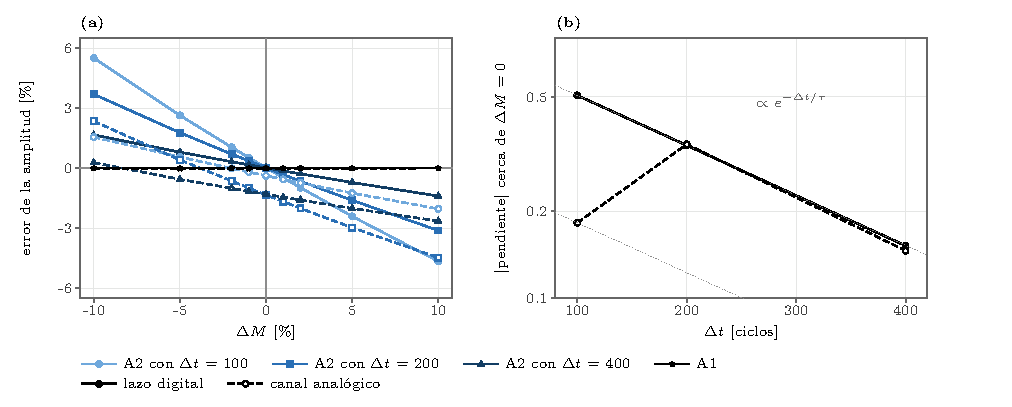
\includegraphics{cap9_meritos_polo_cero}
\caption[Ajuste del polo-cero del trapecio en el lazo digital]{%
Ajuste del polo-cero del trapecio en el lazo digital: pares de 4000 y 2400~ADU
con $\tau = 250$ muestras, separados $\Delta t = 100$, 200 y 400 ciclos, 1000
pares por punto, disparo por polo-cero y la $M$ del trapecio corrida $\Delta M$
entre $-10$ y $+\qty{10}{\percent}$ de la del generador. (a) El error de la
amplitud de $A_2$; (b) la pendiente cerca de $\Delta M = 0$ baja como
$e^{-\Delta t/\tau}$, como la cola de $A_1$ debajo de
$A_2$.\label{f:res-polo-cero}}
\end{figure}

\subsection{Medición de deriva del canal analógico}
\label{S:res-deriva}

Para medir la deriva del canal analógico, alternamos líneas de 1500 y 4000~ADU
cada 3000 ciclos, sin apilamiento, y medimos un punto por minuto durante
\qty{2}{\hour}, con 83\,332 pulsos por punto. En cada punto leímos la
temperatura del Zynq (XADC). Con las dos líneas separamos la deriva en \emph{offset} y
ganancia.

Los resultados se presentan en la Fig.~\ref{f:res-deriva}: en \qty{2}{\hour} la
ganancia recorre 210~ppm, con una pendiente de $-40$~ppm/h. Las líneas recorren
0.8~ADU (la de 1500) y 1.1~ADU (la de 4000), y el \emph{offset} 0.6~ADU. De un minuto
al siguiente las líneas saltan unas 0.12~ADU, 15 veces el error estadístico de
cada punto (0.008~ADU). La temperatura fue de 41.8 a \qty{42.7}{\degreeCelsius},
salvo el primer punto, a \qty{43.2}{\degreeCelsius}. Contra ella la ganancia da
$-144$~ppm/\unit{\degreeCelsius}, con $r = -0.65$. Con un rango de
\qty{1}{\degreeCelsius}, haría falta variar la temperatura a propósito para
separar la temperatura del tiempo.

\begin{figure}[H]
\centering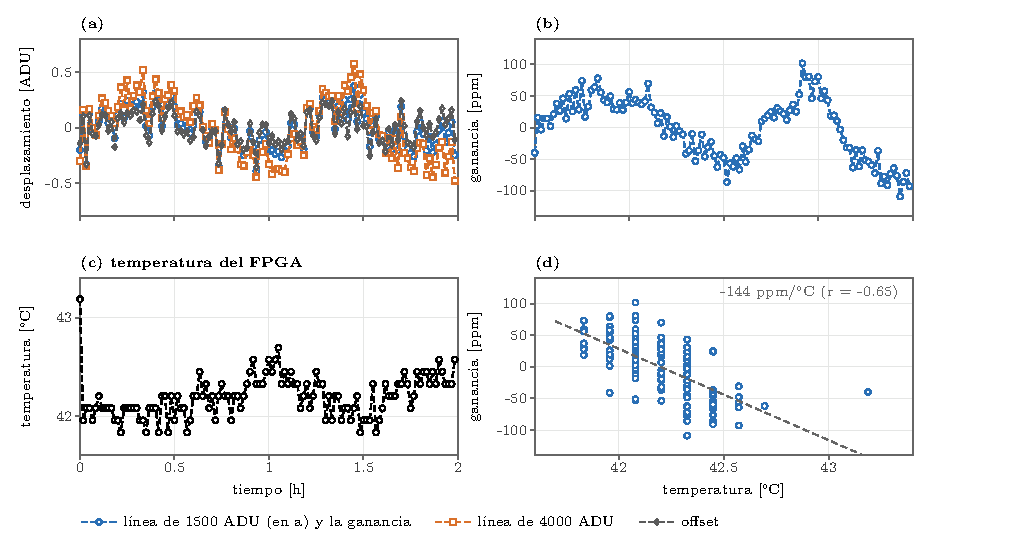
\includegraphics{cap9_meritos_deriva}
\caption[Deriva del canal analógico en 2 h]{%
Deriva del canal analógico en \qty{2}{\hour}: líneas de 1500 y 4000~ADU
alternadas cada 3000 ciclos, 83\,332 pulsos por punto, un punto por minuto, y la
temperatura del Zynq (XADC).\label{f:res-deriva}}
\end{figure}

%==============================================================================
\section{\emph{Throughput} para el osciloscopio}
\label{S:res-throughput-osc}

Como el cambio principal del OSC en este trabajo fue el camino de datos, es la
única propiedad que vamos a describir para este módulo.

La velocidad de registro de eventos se compone de varias operaciones: (1) el
ciclo de lectura de un evento, (2) la agrupación de eventos en un archivo y (3)
la escritura del archivo. La (1) está dada por el HW y la librería de SW, la (2)
únicamente por el SW y la (3) por la capacidad de salida de datos, que puede ser
escritura a la SD o de red. Estas diferencias se presentan en el
Cap.~\ref{C:sw}. En la Fig.~\ref{f:res-throughput} se comparan los siguientes
caminos del \codigo{event\_ring}, que nombramos por el destino de los eventos:
\begin{itemize}
\item DDR: la escritura a DDR.
\item Lector del ring: el lector de C del ring corrido sin guardado en memoria
  secundaria (Sec.~\ref{S:sw-bench-libmca}).
\item SD: el OSC a la SD de la placa por el SW en formato \ruta{.npz}, presentado
  en la Sec.~\ref{S:sw-guardado}.
\item Red: el OSC a la PC por la red.
\end{itemize}
A estos les
sumamos el camino original del osciloscopio, la lectura de la BRAM, con dos
lectores: el lazo de C de \codigo{libmca} y el original, librp desde Python.
Como referencia ponemos el MCA, que no guarda muestras sino que acumula el
espectro en la FPGA.

Llamamos \textbf{techo} de una etapa a la tasa máxima de eventos que puede
sostener cuando la entrada le sobra, es decir, lo que pasa por ella cuando está
saturada. Mientras la entrada está por debajo del techo, la etapa entrega todo
lo que recibe; por encima, entrega su techo y el resto de los eventos se pierde.
Cada etapa tiene el suyo: el de la captura lo fija el HW, el del lector el SW y
el de la red y la SD su ancho de banda.

El techo de la captura sale de su tiempo muerto. Al aceptar un \emph{trigger},
la captura saca la ventana a un canal por ciclo y mientras tanto los
\emph{triggers} nuevos se pierden. Con 2 canales y $S$ = pre + post muestras,
dos eventos tienen que estar separados al menos $2S+3$ ciclos
(Sec.~\ref{S:osc-window-capture}). Con $S=32$ son 67 ciclos de
\qty{8}{\nano\second}, \qty{536}{\nano\second}, y el techo es
$1/\qty{536}{\nano\second}$ $\approx$ 1.87~M/s; con $S=1024$ son 2051 ciclos y el
techo baja a 61~k/s. Con arribos de Poisson la captura se comporta como un
tiempo muerto no paralizable, $m = n/(1+n\tau)$: con $n=3$~M/s y
$\tau=\qty{536}{\nano\second}$ da 1.15~M/s, que es lo que medimos en la DDR.

Las líneas punteadas son los techos. En (a), \codigo{red} y \codigo{SD} son los
techos de cada destino medidos con el ring lleno. En (b), \codigo{captura sola}
es el techo de la captura por su tiempo muerto de $2S+3$ ciclos,
\codigo{TCP solo} el techo por la velocidad de conexión TCP medida con la placa
utilizada (50~MB/s) y \codigo{MCA a 3 M/s} es la tasa
con la que nos comparamos. La recta \codigo{salida = entrada} es la medición
ideal.

\begin{figure}[H]
\centering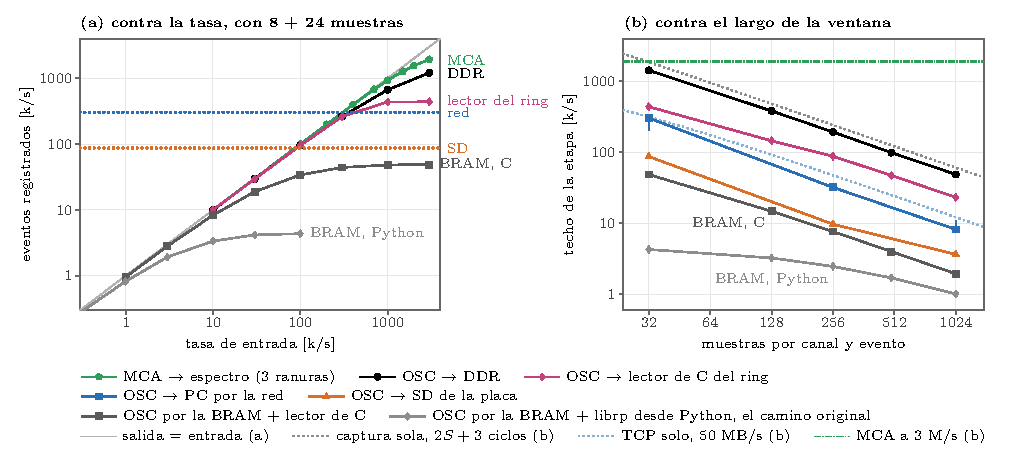
\includegraphics{cap9_throughput_caminos}
\caption[Eventos registrados por segundo en los dos caminos de datos]{%
Eventos registrados por segundo en los dos caminos de datos, medidos en la placa
con generación interna: el MCA, que acumula el espectro en la FPGA, y el
osciloscopio, por el \codigo{event\_ring} o por la BRAM. (a) Tasas
medidas contra las de entrada, con ventanas de 8 + 24 muestras. (b) Techo de
cada etapa contra el largo de la ventana.\label{f:res-throughput}}
\end{figure}

En la Fig.~\ref{f:res-throughput}.a vemos cómo cada etapa recorta la capacidad
de adquisición. Todos los caminos siguen la recta ideal mientras la entrada está
por debajo de su techo y después se aplanan. A 3~M/s de entrada el MCA
registra 1.9~M/s, la captura pone 1.2~M/s en la DDR, el lector
de C del ring lee todo hasta 300~k/s de entrada y se queda en
439~k/s, a la PC por la red llegan 0.3~M/s y a la SD
87~k/s. Cada etapa sostiene lo que le pasa la anterior hasta su propio
techo, así que el camino completo queda fijado por la etapa más lenta. Esto
viene de que tenemos mayor \emph{throughput} para escribir memoria primaria que
secundaria: la DDR acepta lo que captura el HW, mientras que la SD, limitada por
el bus del controlador del Zynq, es la etapa más lenta, y la red queda en el
medio.

La velocidad de adquisición tiene como techo fijo el sistema presentado en HW,
pero ese techo no es el que limita: con ventanas cortas la captura pasa
1.4~M/s y lo que se guarda de forma persistente es entre 5 y 16 veces
menos. En la Fig.~\ref{f:res-throughput}.b vemos que al alargar la ventana
todos los techos bajan. La captura pierde por su tiempo muerto, el lector de C
queda un poco abajo y la red y la SD bajan como su ancho de banda sobre los
bytes por evento ($32+4S$): con 1024 muestras la DDR pasa 49~k/s, el
lector 23~k/s, la red 8.2~k/s y la SD 3.7~k/s. Para el MCA
el largo de la ventana no importa, porque no guarda muestras: este es el motivo
por el que, a igual tasa de entrada, el MCA siempre registra más eventos que el
osciloscopio.

La mejora presente por el osciloscopio se presenta en la comparación con el
camino original por la BRAM, que se lee palabra a palabra por el bus. Con
ventanas de 32 muestras, librp desde Python llega a 4.4~k/s y el lector
de C de la BRAM a 49~k/s, mientras que el lector de C del ring lee
439~k/s: \textbf{100 veces el camino original} y 9 veces el mismo lector
sobre la BRAM. Aún guardando los eventos, por la red llegan 0.3~M/s, unas
70 veces el camino original sin guardar. Con 1024 muestras la diferencia se
achica, porque domina el volumen de datos: el lector del ring pasa
23~k/s contra 1.0~k/s de Python y 2.0~k/s del lector de C
sobre la BRAM.

%%% Local Variables:
%%% mode: latex
%%% TeX-master: "template"
%%% End:
